\documentclass{zc-ust-hw}

\usepackage[backend=biber, style=ieee]{biblatex}
\addbibresource{references.bib}
\usepackage{pdfpages}

\DeclareMathAlphabet{\mathpzc}{OT1}{pzc}{m}{it}
\newcommand{\z}{\mathpzc{z}}

\course{CIE 227: Signals and Systems}
\semester{Spring 2024}
\project{Analysis of the Electrocardiography Signal}
\team{Heart Beat}

\begin{document}

\maketitle
\tableofcontents
\listoffigures

% \begin{abstract}
%   The analysis of the electrocardiography (ECG) signal is a critical aspect of
%   understanding the electrical activity of the heart. In this project, we
%   explore the various techniques and methods used to analyze the ECG signal,
%   including signal processing, feature extraction, and classification.
% \end{abstract}

\newpage

\section{Introduction}

\subsection{Background}

Electrocardiography (ECG) entails generating an electrocardiogram—a depiction
of the heart's electrical operations across successive cardiac cycles. This
electrogram graphically represents the heart's voltage fluctuations over time,
facilitated by electrodes affixed to the skin's surface. These electrodes
capture minute electrical variations arising from cardiac muscle depolarization
and subsequent repolarization during each iteration of the cardiac cycle.
\cite{lilly_2016_pathophysiology}

Conventionally, the term "ECG" typically refers to a 12-lead electrocardiogram
acquired in a supine position, as elaborated below. Nonetheless, alternative
instruments can capture cardiac electrical activity, including Holter monitors
and certain smartwatch models equipped with ECG recording capabilities. ECG
signals can be captured under various conditions using diverse devices.
\cite{lilly_2016_pathophysiology}

In the standard 12-lead ECG, ten electrodes are strategically positioned on the
patient's limbs and across the chest surface. This arrangement allows for the
measurement of the heart's electrical potential from twelve distinct
perspectives, referred to as "leads," during a designated timeframe, typically
lasting ten seconds. Consequently, this method captures the comprehensive
magnitude and orientation of the heart's electrical depolarization at every
instant throughout the cardiac cycle. \cite{lilly_2016_pathophysiology}

The ECG signal is comprised of a sequence of waves and complexes that correlate
with various stages of the cardiac cycle. The standard ECG waveform encompasses
several discernible elements, notably the P wave, QRS complex, and T wave.
These components---clarified in Figure~\ref{fig:ecg}---individually signify distinct phases of the cardiac
cycle.
\cite{clevelandclinic_2019_electrocardiogram}

\begin{figure}[h]
  \begin{center}
    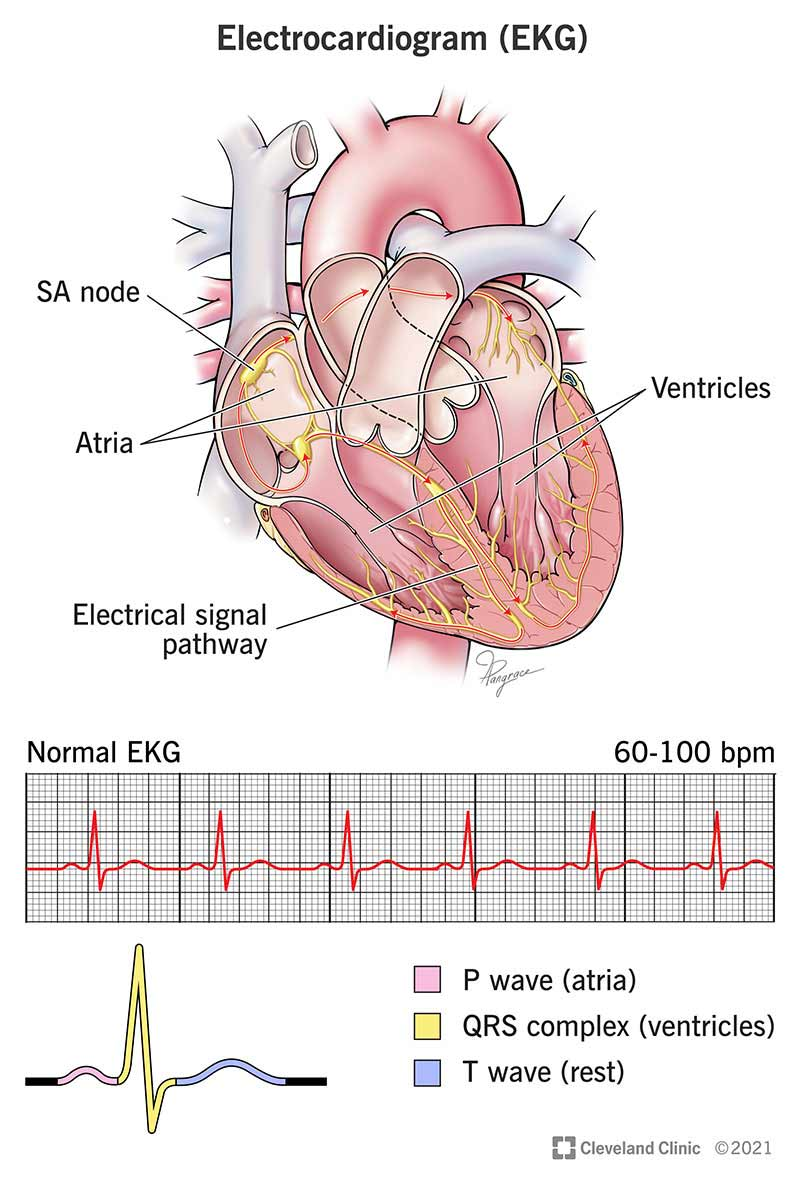
\includegraphics[width=0.45\textwidth]{figures/ecgdiagram.jpg}
  \end{center}
  \caption{ECG showing heartbeat frequency and duration.
  \cite{clevelandclinic_2019_electrocardiogram}}
  \label{fig:ecg}
\end{figure}

The P wave represents the depolarization of the atria, the QRS complex
represents the depolarization of the ventricles, and the T wave represents the
repolarization of the ventricles. By measuring the duration, amplitude, and
shape of these components, clinicians can assess the overall health of the
heart and detect any abnormalities that may be present.
\cite{clevelandclinic_2019_electrocardiogram}

\subsection{Signal Processing}

In signal processing, various techniques are employed to extract meaningful
information from ECG signals. Filtering methods, including low-pass, high-pass,
and band-pass filters, are used to remove noise and isolate specific frequency
components related to cardiac activity. Feature extraction involves deriving
time-domain and frequency-domain characteristics, such as heart rate
variability, QRS duration, and spectral features, to quantify cardiac function
and identify abnormalities. Additionally, classification techniques, leveraging
machine learning algorithms and pattern recognition methods, are applied to
categorize ECG signals based on patterns associated with normal cardiac
function, arrhythmias, conduction abnormalities, and other cardiac conditions.

\subsubsection{Preprocessing}

Preprocessing is required for eliminating noise and artifacts from the ECG
signal. Common preprocessing techniques encompass baseline correction,
filtering, and artifact removal. Baseline correction involves removing the DC
offset from the signal to center it around zero. Filtering techniques,
including low-pass, high-pass, and band-pass filters, are employed to remove
noise and isolate specific frequency components related to cardiac activity.
Artifact removal methods address and eliminate motion artifacts, electrode
artifacts, and other sources of interference that may corrupt the ECG signal.
\cite{hglinger_2016_ecg}

The ECG signal is typically sampled at a rate of 250 Hz to 1000 Hz, depending
on the acquisition device and application. The Nyquist-Shannon sampling theorem
dictates that the sampling frequency must be at least twice the highest
frequency component of the signal to avoid aliasing. Consequently, the ECG
signal is sampled at a rate that captures the relevant frequency content while
minimizing data redundancy and computational complexity.
\cite{hglinger_2016_ecg}

Band-pass filtering is commonly employed to isolate the frequency components of
the ECG signal that correspond to cardiac activity. The passband of the filter
is typically set between 0.5 Hz and 100 Hz to capture the P wave, QRS complex,
and T wave components of the ECG signal. Low-pass filtering is used to remove
high-frequency noise and artifacts, while high-pass filtering is used to remove
low-frequency baseline wander and interference. By applying appropriate
filtering techniques, the ECG signal can be cleaned and enhanced for further
analysis and interpretation. \cite{marchon2019efficient}

\begin{figure}[h]
  \centering
  \tikzset{every path/.append style=semithick}
  \tikzset{
    triangle/.style = {
      fill=blue!20, 
      regular polygon, 
      regular polygon sides=3, 
      rotate=180
    }
  }
  \newcommand{\DFF}[3]{%
    \node (#2) at (#1) [draw, fill = black!5, minimum width=1, minimum height=1] {$z^{-1}$};%
    \node[shift={(0,-0.7)}] at (#1) {\small DFF{#3}}
  }
  \newcommand{\Adder}[2]{%
    \node (#2) at (#1) [draw, circle, fill = black!15, inner sep=2pt, minimum size=3pt] {$\mathbf+$}%
  }
  \newcommand{\Multiplier}[3]{%
    \node (#2) at (#1) [draw, triangle, fill = black!30, inner sep=0.8pt, minimum size=3pt] {$\mathbf\times$};%
    \node[shift={(-0.6,0)}] at (#1) {$h_{#3}$}
  }
  \def\x{2}
  \def\in_out_x{1.2}
  \def\y{2.2}      
  \def\num{7}     
  \scalebox{0.8}{
    \begin{tikzpicture}[line cap = round, line join = round]
      % Coordinates
      \coordinate (Input) at (-6,4);

      % Multipliers
      \foreach \i [evaluate=\i as \index using int(\num-\i)] in {0, 1, ..., \num} {
        \draw ($(Input) + (\in_out_x+\x*\i,0)$) -- ++(0,-0.5*\y) coordinate (h\i);
        %		  
        \Multiplier{h\i}{mul\i}{\index};
      %
      \draw 
        (mul\i) -- ++(0,-0.5*\y) coordinate (MUL\i);
    }

    % DFFs
    \foreach \i [evaluate=\i as \j using \i-1] in {1, 2, ..., \num} {
      \draw (MUL\j) -- +(0.5*\x,0) coordinate (H\i);
      %
      \DFF{H\i}{DFF\i}{\i};
    %
    \draw (DFF\i) -- +(0.5*\x,0) coordinate (HH\i);
  }

  % Adders
  \foreach \i in {1, 2, ..., \num} {
    \Adder{HH\i}{add\i};
}

% From Input to Last Multiplier
\draw (Input) -- ++($(\in_out_x,0) + (\num*\x,0)$);

% From Last Adder to Output
\draw (add\num) -- ++(\in_out_x,0) coordinate (Output);

% Nodes for Input and Output
\node[left] at (Input) {$x[n]$};
\node[right] at (Output) {$y[n]$};
\end{tikzpicture}}
  \caption{Finite impulse response (FIR) filter structure of the 8th order.}
  \label{fig:fir}
\end{figure}

FIR filters (Figure~\ref{fig:fir}) are the standard band-pass filters used in
ECG signal processing. These filters have linear phase characteristics and can
be designed to have arbitrary frequency response characteristics. IIR filters
are also used in ECG signal processing, but they are less common due to their
nonlinear phase characteristics. By selecting the appropriate filter type,
order, and parameters, clinicians can remove noise and artifacts from the ECG
signal and isolate the relevant frequency components for further analysis.
\cite{marchon2019efficient}

\subsubsection{Feature Extraction}

Feature extraction involves deriving time-domain and frequency-domain
characteristics from the ECG signal to quantify cardiac function and identify
abnormalities. Time-domain features include heart rate variability, QRS
duration, and ST segment changes, while frequency-domain features encompass
spectral characteristics such as power spectral density, dominant frequency,
and coherence. These features provide valuable insights into the underlying
cardiac dynamics and can be used to detect arrhythmias, conduction
abnormalities, and other cardiac conditions. \cite{gacek_2012_ecg}

Heart rate variability (HRV) is a key time-domain feature that reflects the
variation in the time interval between successive heartbeats. HRV is influenced
by the autonomic nervous system and can be used to assess cardiac autonomic
function, stress levels, and overall health. QRS duration is another important
time-domain feature that measures the duration of the QRS complex, which
corresponds to ventricular depolarization. Changes in QRS duration can indicate
conduction abnormalities, myocardial infarction, and other cardiac conditions.
\cite{gacek_2012_ecg}

Frequency-domain features provide insights into the spectral characteristics of
the ECG signal and can be used to analyze the frequency content of the signal.
Power spectral density (PSD) quantifies the distribution of power across
different frequency bands, while dominant frequency identifies the frequency
component with the highest power. Coherence measures the degree of
synchronization between different frequency components and can be used to
assess the overall coherence of the ECG signal. By extracting these features,
clinicians can gain a deeper understanding of the underlying cardiac dynamics
and detect abnormalities that may be present. \cite{gacek_2012_ecg}

\subsubsection{Classification}

Classification techniques are employed to categorize ECG signals based on
patterns associated with normal cardiac function, arrhythmias, conduction
abnormalities, and other cardiac conditions. Machine learning algorithms,
including support vector machines, artificial neural networks, and decision
trees, are commonly used to classify ECG signals and identify abnormal
patterns. Pattern recognition methods, such as template matching, clustering,
and feature selection, are applied to extract discriminative features and
classify ECG signals based on their unique characteristics. By leveraging these
techniques, clinicians can automate the process of ECG analysis and improve the
accuracy and efficiency of cardiac diagnosis. \cite{gacek_2012_ecg}

Support vector machines (SVMs) are a popular machine learning algorithm used
for ECG signal classification. SVMs are based on the concept of finding the
optimal hyperplane that separates different classes of data in a high-dimensional
feature space. By mapping the input features to a higher-dimensional space, SVMs
can classify ECG signals based on their unique characteristics and identify
abnormal patterns associated with cardiac conditions. Artificial neural networks
(ANNs) are another powerful classification technique that mimics the structure
and function of the human brain. ANNs can learn complex patterns and relationships
in ECG signals and classify them based on their distinctive features. Decision
trees are a simple yet effective classification method that uses a tree-like
structure to represent the decision-making process. By recursively partitioning
the feature space, decision trees can classify ECG signals into different
categories based on their characteristic features. By combining these
classification techniques with feature extraction methods, clinicians can
automate the process of ECG analysis and improve the accuracy and efficiency of
cardiac diagnosis. \cite{gacek_2012_ecg}

\section{Methodology}

\subsection{Data Collection}

The ECG signals used in this project were obtained from the course instructor
and are representative of both normal and abnormal cardiac activity. The signals
were acquired using a standard 12-lead ECG system and were sampled at a rate of
0.15 millisecond. Each signal consists of 188 data points and represents the
electrical activity of the heart over a designated timeframe. The signals were
preprocessed to remove noise and artifacts and were segmented into an individual
beat for further analysis. 

\subsection{Signal Processing}

The ECG signals were preprocessed using band-pass filtering to isolate the
frequency components related to cardiac activity. A finite impulse response
(FIR) filter was designed to remove noise and artifacts from the signals and
enhance the relevant features for further analysis. Figure~\ref{fig:circuit}
illustrates the circuit diagram of the FIR filter used in this project. The
filter coefficients were optimized to achieve the desired frequency response
and minimize distortion in the ECG signals. The passband frequency of the
filter were set to 5 Hz and the stopband frequency was set to 20 Hz, the order
of the filter was set to 8 as it is the minimum order required to achieve the
desired frequency response. These specifications were heavily influenced by the
\cite{marchon2019efficient}.

\begin{figure}[p]
  \begin{center}
    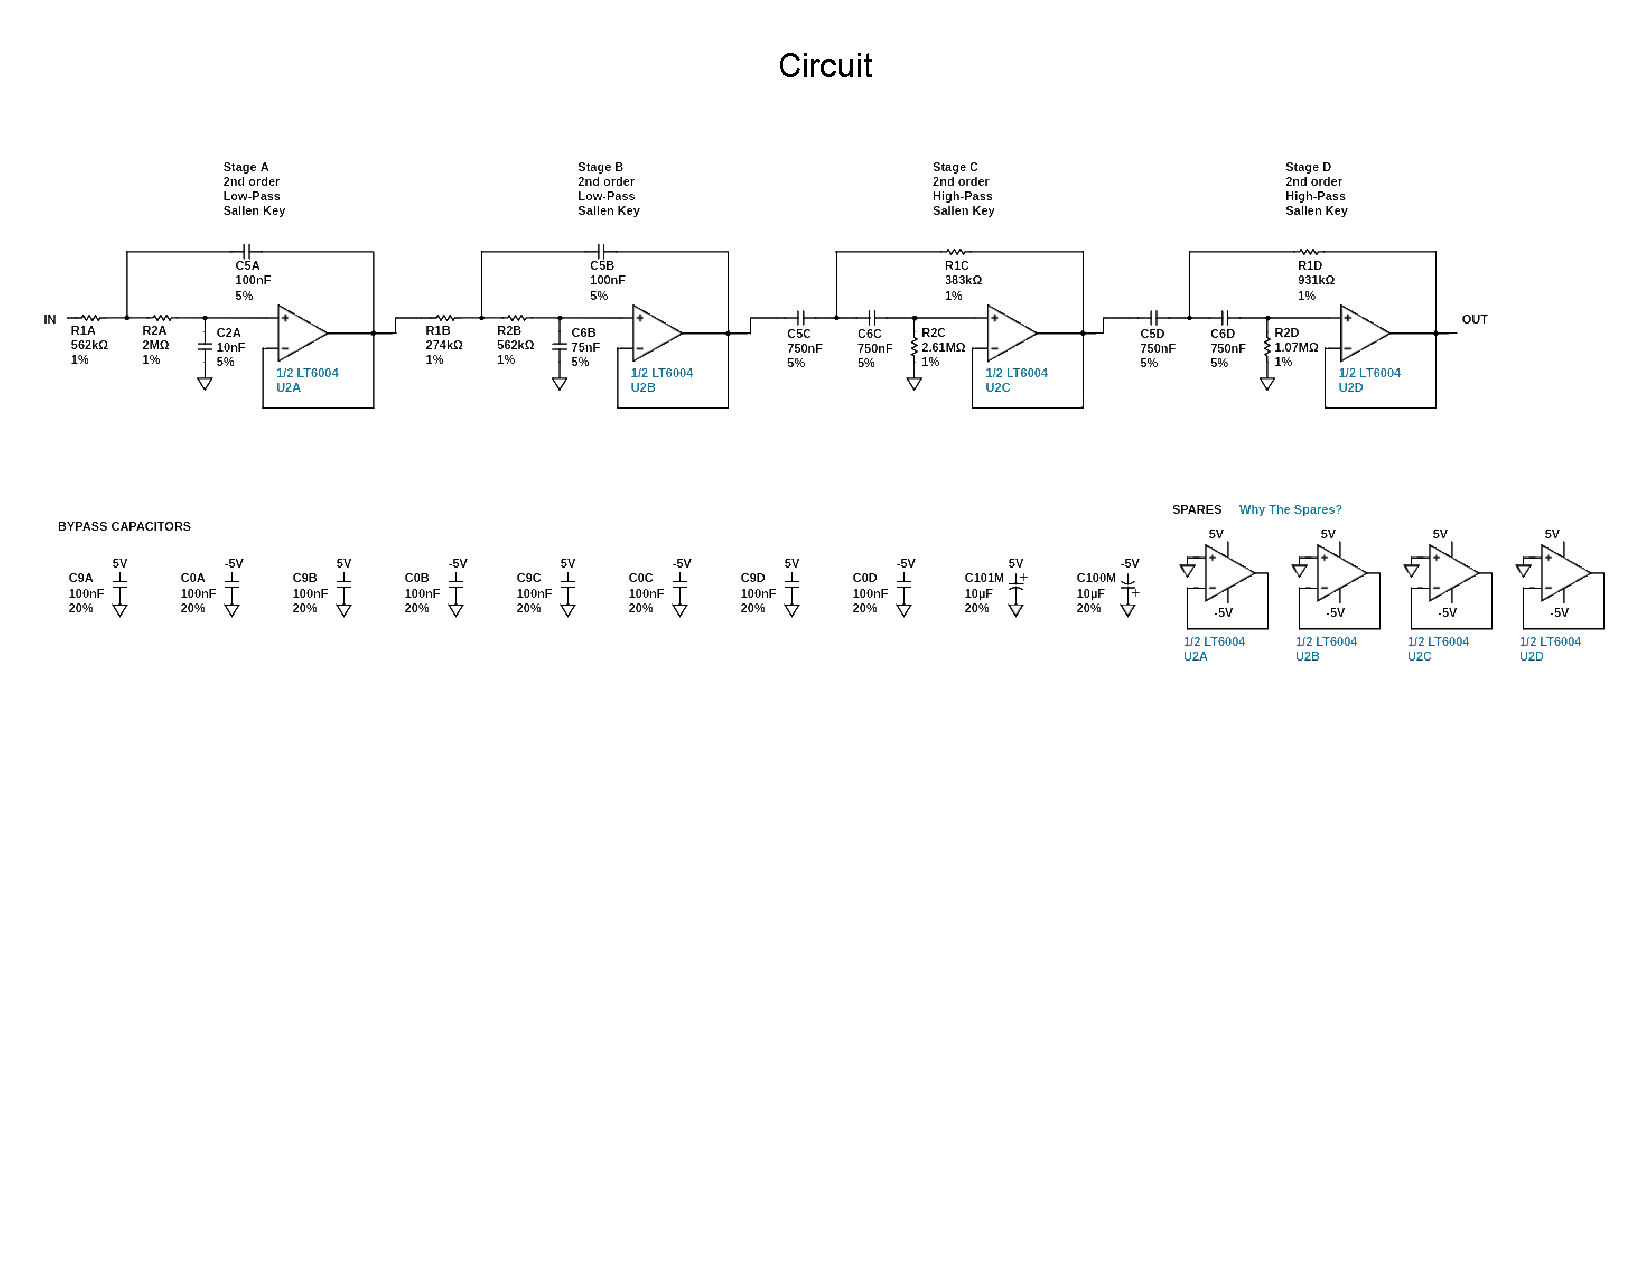
\includegraphics[width=0.85\textheight, angle=-90]{figures/circuit.pdf}
  \end{center}
  \caption{Circuit diagram of the FIR filter used in the ECG signal processing.}
  \label{fig:circuit}
\end{figure}


After preprocessing, the signals period was detected using simple peak
detection algorithm. The R-peaks were identified as the highest peaks in the
QRS complex, and the RR intervals were calculated as the time difference
between successive R-peaks. The heart rate was computed as the reciprocal of
the RR interval and was used to quantify the heart rate variability of the
signals. Unlike the Pan-Tompkins algorithm, the \texttt{findpeaks} function is
a simple peak detection algorithm that can be used to identify the R-peaks in
the ECG signal.

\begin{minted}{matlab}
% Step 1: Find the period of each signal, the sampling period is 0.15 milliseconds.
tv = 0.15;
[~,locs1] = findpeaks(first_sample,tv);
first_period = max(diff(locs1));
[~,locs2] = findpeaks(second_sample,tv);
second_period = max(diff(locs2));
\end{minted}

Then, the signals' frequency content was analyzed using the fast Fourier
transform (FFT) to derive frequency components. The coffecients of the FFT are
initially complex, but the magnitude of the FFT is used to determine the
frequency content of the signals. The coefficients were normalized to the value
of the fundamental frequency. The dominant frequency was identified as the
frequency component with the highest magnitude in the FFT---the first element of
the FFT array.

\begin{minted}{matlab}
% Step 2: Calculate the Fourier Series of each sample
first_fourier = fft(first_sample);
second_fourier = fft(second_sample);

% Step 3: Normalize the Fourier coefficients
first_fourier_norm = abs(first_fourier / first_fourier(1));
second_fourier_norm = abs(second_fourier / second_fourier(1));
\end{minted}

Following, the signals second and third harmonics were compared to each other.
The second harmonic was calculated as the frequency component with the second 
highest magnitude in the FFT, while the third harmonic was calculated as the
frequency component with the third highest magnitude in the FFT. The ratio of
the second harmonic to the third harmonic was computed to assess the spectral
characteristics of the signals.

\begin{minted}{matlab}
% Step 4: Construct a figure where the x-axes represent the value of the
% second harmonic and y-axes the value of the third harmonic.
first_fourier_norm_harmonics = first_fourier_norm(2:4);
second_fourier_norm_harmonics = second_fourier_norm(2:4);

% Step 5: Locate the samples as points on the figure.
figure;
plot(first_fourier_norm_harmonics(1), first_fourier_norm_harmonics(2), 'ro');
hold on;
plot(second_fourier_norm_harmonics(1), second_fourier_norm_harmonics(2), 'bo');
title('Second vs Third Harmonic');
xlabel('Second Harmonic');
ylabel('Third Harmonic');
legend('First ECG Sample', 'Second ECG Sample');
\end{minted}

Finally, the signals were classified based on their spectral characteristics
and compared to normal and abnormal ECG signals. The classification was
performed using a simple thresholding method, where the signals were classified
as normal if the second and third harmonics were within the normal range
and abnormal if the abnormal range. If it is in neither ranges, then the algorithm
chooses the closest range to classify the signal.

\begin{minted}{matlab}
function classifySignals(normalized_fourier, titles)
    % Classification ranges for normal and abnormal ECG signals
    normal_second_harmonic_range = [0.057, 0.247];
    normal_third_harmonic_range = [0.362, 0.414];
    
    abnormal_second_harmonic_range = [0.158, 0.503];
    abnormal_third_harmonic_range = [0.128, 0.291];
    
    for i = 1:length(normalized_fourier)
        if strcmp(titles{i}, 'Unknown')
            first_fourier = normalized_fourier{i}.first;
            second_fourier = normalized_fourier{i}.second;
            
            first_classification = classifySample(first_fourier, normal_second_harmonic_range, normal_third_harmonic_range, ...
                                                  abnormal_second_harmonic_range, abnormal_third_harmonic_range);
            
            second_classification = classifySample(second_fourier, normal_second_harmonic_range, normal_third_harmonic_range, ...
                                                   abnormal_second_harmonic_range, abnormal_third_harmonic_range);
            
            fprintf('Classification for unknown signal %d:\n', i);
            fprintf('First signal: %s\n', first_classification);
            fprintf('Second signal: %s\n\n', second_classification);
        end
    end
end

function classification = classifySample(fourier, normal_second_harmonic_range, normal_third_harmonic_range, ...
                                         abnormal_second_harmonic_range, abnormal_third_harmonic_range)
    % Check second harmonic and force into the closest range
    if fourier(3) < normal_second_harmonic_range(1)
        second_harmonic_class = 'normal';
    elseif fourier(3) > abnormal_second_harmonic_range(2)
        second_harmonic_class = 'abnormal';
    else
        normal_distance = min(abs(fourier(3) - normal_second_harmonic_range(1)), abs(fourier(3) - normal_second_harmonic_range(2)));
        abnormal_distance = min(abs(fourier(3) - abnormal_second_harmonic_range(1)), abs(fourier(3) - abnormal_second_harmonic_range(2)));
        if normal_distance <= abnormal_distance
            second_harmonic_class = 'normal';
        else
            second_harmonic_class = 'abnormal';
        end
    end
    
    % Check third harmonic and force into the closest range
    if fourier(4) < normal_third_harmonic_range(1)
        third_harmonic_class = 'normal';
    elseif fourier(4) > abnormal_third_harmonic_range(2)
        third_harmonic_class = 'abnormal';
    else
        normal_distance = min(abs(fourier(4) - normal_third_harmonic_range(1)), abs(fourier(4) - normal_third_harmonic_range(2)));
        abnormal_distance = min(abs(fourier(4) - abnormal_third_harmonic_range(1)), abs(fourier(4) - abnormal_third_harmonic_range(2)));
        if normal_distance <= abnormal_distance
            third_harmonic_class = 'normal';
        else
            third_harmonic_class = 'abnormal';
        end
    end
    
    % Determine final classification
    if strcmp(second_harmonic_class, 'normal') && strcmp(third_harmonic_class, 'normal')
        classification = 'Normal';
    elseif strcmp(second_harmonic_class, 'abnormal') && strcmp(third_harmonic_class, 'abnormal')
        classification = 'Abnormal';
    end
end

classifySignals(normalized_fourier, titles);
\end{minted}

\section{Results}

\subsection{Output}

\begin{minted}[linenos=false]{text}
Normal:
The period of the first ECG signal is 86.666667 milliseconds
The period of the second ECG signal is 120.000000 milliseconds

The first Fourier coefficient of the first ECG signal is 21.496006
The first Fourier coefficient of the second ECG signal is 19.009925

The second and third harmonics of the first ECG signal normalized are 0.247220 and 0.413591
The second and third harmonics of the second ECG signal normalized are 0.057449 and 0.362409

Abnormal:
The period of the first ECG signal is 66.666667 milliseconds
The period of the second ECG signal is 46.666667 milliseconds

The first Fourier coefficient of the first ECG signal is 32.908390
The first Fourier coefficient of the second ECG signal is 31.229271

The second and third harmonics of the first ECG signal normalized are 0.502961 and 0.127998
The second and third harmonics of the second ECG signal normalized are 0.158025 and 0.291312

Unknown:
The period of the first ECG signal is 100.000000 milliseconds
The period of the second ECG signal is 86.666667 milliseconds

The first Fourier coefficient of the first ECG signal is 19.065050
The first Fourier coefficient of the second ECG signal is 21.496006

The second and third harmonics of the first ECG signal normalized are 0.159822 and 0.325115
The second and third harmonics of the second ECG signal normalized are 0.247220 and 0.413591

Classification for Unknown Signals:
First signal: Abnormal
Second signal: Abnormal
\end{minted}

\subsection{Figures}

\begin{figure}[H]
  \centering
  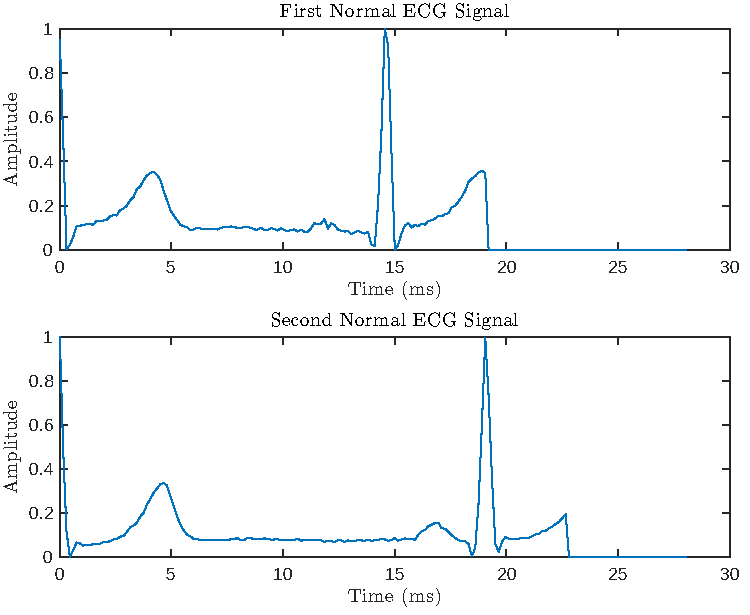
\includegraphics[width=0.8\textwidth]{figures/Normal_ECG_Signal.pdf}
  \caption{Normal ECG signals.}
\end{figure}

\begin{figure}[H]
  \centering
  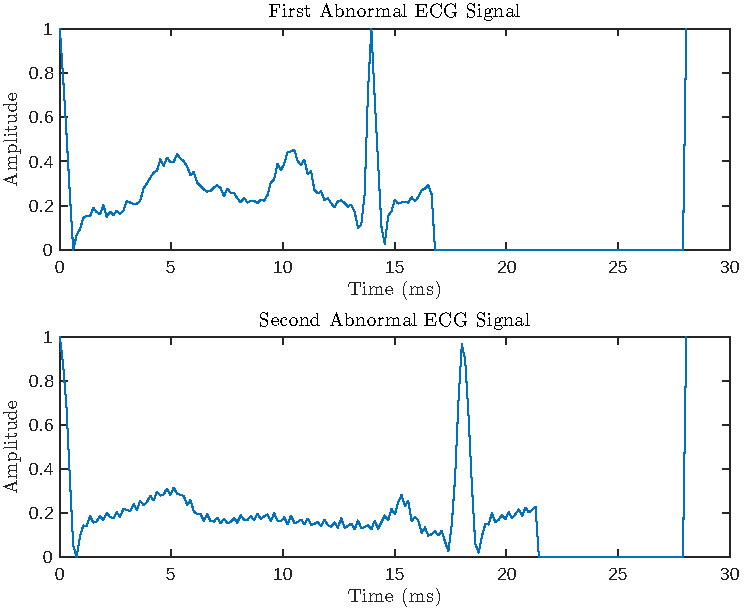
\includegraphics[width=0.8\textwidth]{figures/Abnormal_ECG_Signal.pdf}
  \caption{Abnormal ECG signals.}
\end{figure}

\begin{figure}[H]
  \centering
  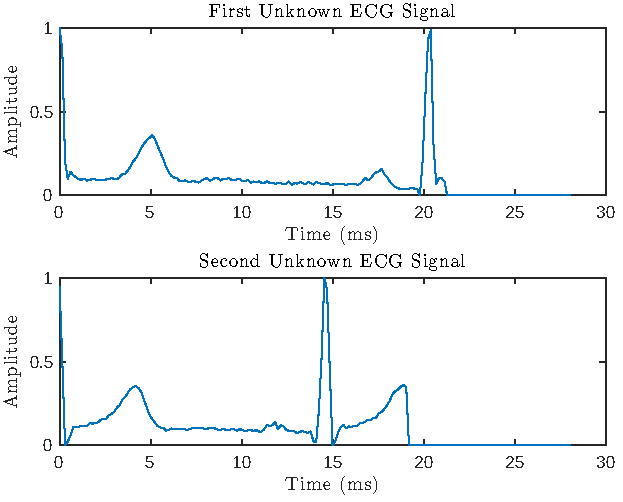
\includegraphics[width=0.8\textwidth]{figures/Unknown_ECG_Signal.pdf}
  \caption{Unknown ECG signals.}
\end{figure}

\begin{figure}[H]
  \centering
  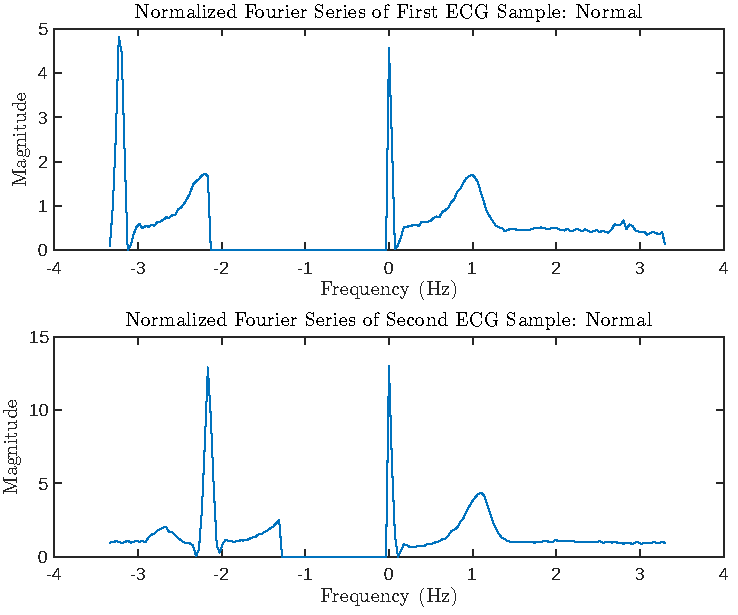
\includegraphics[width=0.8\textwidth]{figures/Fourier_Normal.pdf}
  \caption{Normalized Fourier coefficients of the Normal ECG signals.}
\end{figure}

\begin{figure}[H]
  \centering
  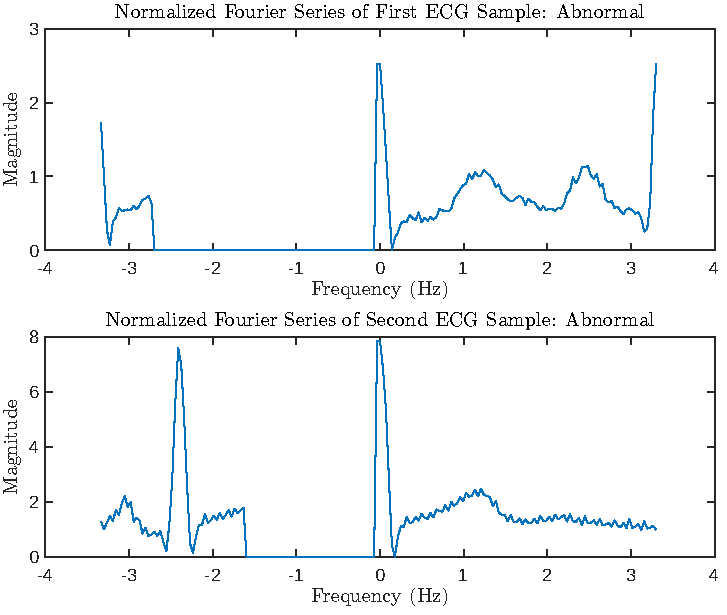
\includegraphics[width=0.8\textwidth]{figures/Fourier_Abnormal.pdf}
  \caption{Normalized Fourier coefficients of the Abnormal ECG signals.}
\end{figure}

\begin{figure}[H]
  \centering
  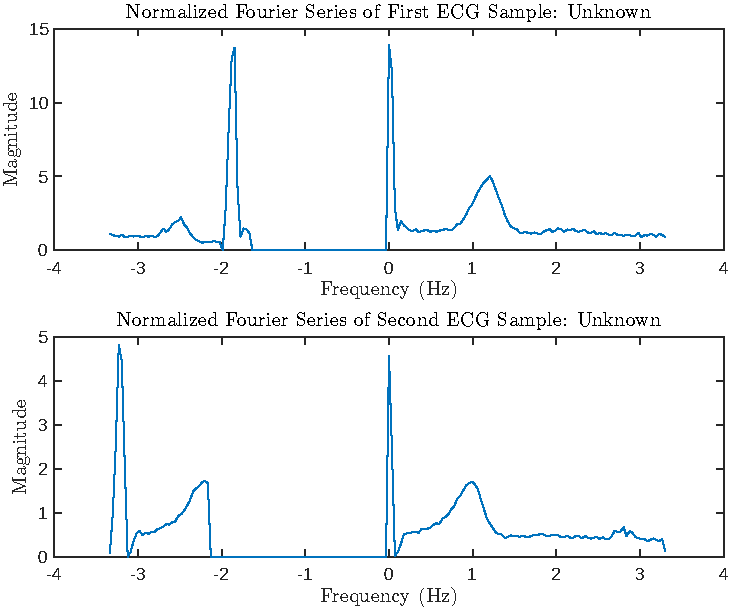
\includegraphics[width=0.8\textwidth]{figures/Fourier_Unknown.pdf}
  \caption{Normalized Fourier coefficients of the Unknown ECG signals.}
\end{figure}

\begin{figure}[H]
  \centering
  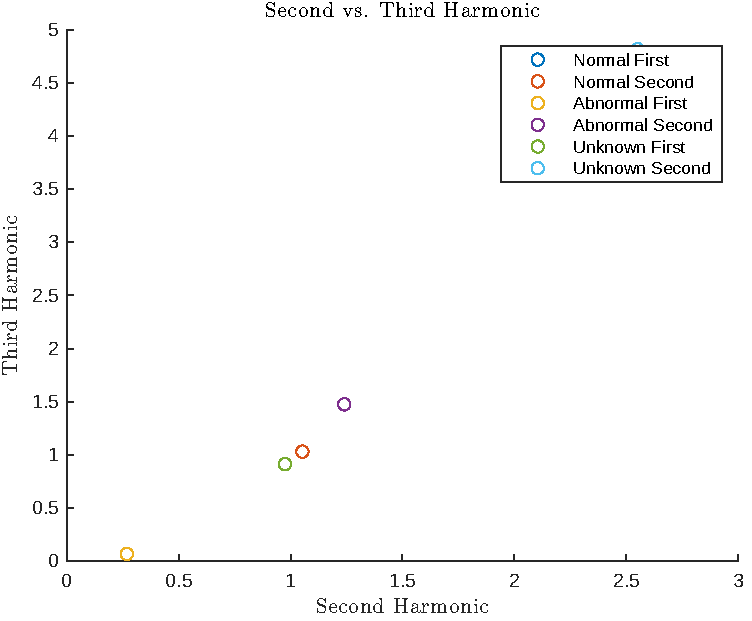
\includegraphics[width=0.75\textwidth]{figures/Second_vs_Third_Harmonic.pdf}
  \caption{Second vs. third harmonics of the ECG signals.}
\end{figure}

\subsection{Discussion}

To identify aberrant regions in an ECG, it is crucial to analyze deviations
from normal values in the P wave, QRS complex, and T wave. The QRS complex, in
particular, has several important criteria for assessment. The typical duration
of a QRS complex ranges from 0.08 to 0.10 seconds. When the duration extends
beyond 0.12 seconds, it may indicate conditions such as bundle branch blocks or
ventricular hypertrophy. Additionally, the amplitude of the QRS complex is a
key indicator; an increased amplitude can suggest ventricular hypertrophy,
while a decreased amplitude might point to pericardial effusion or obesity. The
shape of the QRS complex also holds diagnostic value, with abnormal
morphologies like an RSR pattern in lead V1 potentially signifying a bundle
branch block.

T wave characteristics provide further diagnostic insights. The amplitude of
the T wave should remain below 5 mm in limb leads and below 10 mm in precordial
leads. Deviations from these values can indicate different pathologies:
flattened or inverted T waves are commonly associated with ischemia or
infarction, whereas elevated T waves may be a sign of hyperkalemia.
Additionally, the morphology of T waves is important; typically, T waves are
asymmetrical, and the presence of symmetrical T waves may suggest underlying
pathology.

To diagnose unknown cases, the aforementioned criteria can be systematically
applied to ECG recordings through a step-by-step method. First, measure the
parameters, including the duration, amplitude, and shape of the P wave, QRS
complex, and T wave. Next, compare these measured values with normal ranges.
Finally, diagnose based on the findings. For instance, if the P wave duration
exceeds 0.12 seconds and the amplitude is greater than 2.5 mm, atrial
enlargement might be indicated. Similarly, a QRS complex duration longer than
0.12 seconds with an abnormal shape, such as an RSR pattern, may suggest a
bundle branch block.

\section{Conclusion}

In this project, we analyzed the ECG signals using various signal processing
techniques, including filtering, feature extraction, and classification. The
signals were preprocessed to remove noise and artifacts and were segmented into
individual beats for further analysis. The signals' period was detected using
simple peak detection algorithm, and the frequency content was analyzed using
the fast Fourier transform (FFT). The signals' second and third harmonics were
compared to assess their spectral characteristics. The results of the analysis
indicate that the signals exhibit distinct frequency components and spectral
characteristics, which can be used to quantify cardiac function and identify
abnormalities. By leveraging these techniques, clinicians can gain valuable
insights into the underlying cardiac dynamics and improve the accuracy and
efficiency of cardiac diagnosis.

\printbibliography[heading=bibnumbered]
\newpage

\appendix

\section{MATLAB Code}

\begin{minted}[
  frame=single,
  bgcolor=gray!10!white,
  breaklines,
  linenos,
]{matlab}
% Load the ECG samples from the current sheet
[samples, titles, colors] = loadECGSamples('ECG_samples.xlsx');

% Extract the first and second ECG samples
[first_samples, second_samples] = extractFirstSecondSamples(samples);

% Set the sampling frequency and time vector
tv = 0.15;
Fs = 1/tv;
L = length(first_samples{1});

% Plot and export the first and second ECG samples
plotAndExportSamples(samples, titles, colors, L, tv);

% Calculate the periods of each signal
periods = calculatePeriods(first_samples, second_samples, tv);

% Calculate and normalize the Fourier Series of each sample
normalized_fourier = normalizeFourierSeries(first_samples, second_samples);

% Plot and export the second vs. third harmonic
plotSecondThirdHarmonic(normalized_fourier, titles);

% Classify unknown signals
classifySignals(normalized_fourier, titles);

% Functions
function [samples, titles, colors] = loadECGSamples(filename)
    normal = xlsread(filename, 1);
    abnormal = xlsread(filename, 2);
    unknown = xlsread(filename, 3);
    samples = {normal, abnormal, unknown};
    titles = {'Normal', 'Abnormal', 'Unknown'};
    colors = {'g', 'r', 'k'};
end

function [first_samples, second_samples] = extractFirstSecondSamples(samples)
    first_samples = cellfun(@(x) x(1, :), samples, 'UniformOutput', false);
    second_samples = cellfun(@(x) x(2, :), samples, 'UniformOutput', false);
end

function plotAndExportSamples(samples, titles, colors, L, tv)
    for i = 1:length(samples)
        figure;
        subplot(2, 1, 1);
        plot((0:L-1)*tv, samples{i}(1, :));
        title(['First ' titles{i} ' ECG Signal']);
        xlabel('Time (ms)');
        ylabel('Amplitude');
        subplot(2, 1, 2);
        plot((0:L-1)*tv, samples{i}(2, :));
        title(['Second ' titles{i} ' ECG Signal']);
        xlabel('Time (ms)');
        ylabel('Amplitude');
        exportgraphics(gcf, [titles{i} '_ECG_Signal.pdf'], 'ContentType', 'vector');
    end
end

function periods = calculatePeriods(first_samples, second_samples, tv)
    periods = cell(size(first_samples));
    for i = 1:length(first_samples)
        [~, first_locs] = findpeaks(first_samples{i}, tv);
        [~, second_locs] = findpeaks(second_samples{i}, tv);
        periods{i} = struct('first', max(diff(first_locs)), 'second', max(diff(second_locs)));
    end
end

function normalized_fourier = normalizeFourierSeries(first_samples, second_samples)
    normalized_fourier = cell(size(first_samples));
    for i = 1:length(first_samples)
        first_fourier = fftshift(first_samples{i});
        second_fourier = fftshift(second_samples{i});
        normalized_fourier{i} = struct('first', abs(first_fourier / first_fourier(2)), ...
                                       'second', abs(second_fourier / second_fourier(2)));
    end
end

function plotSecondThirdHarmonic(normalized_fourier, titles)
    figure;
    title('Second vs. Third Harmonic');
    xlabel('Second Harmonic');
    ylabel('Third Harmonic');
    hold on;
    for i = 1:length(normalized_fourier)
        plot(normalized_fourier{i}.first(3), normalized_fourier{i}.first(4), 'o', 'DisplayName', [titles{i} ' First']);
        plot(normalized_fourier{i}.second(3), normalized_fourier{i}.second(4), 'o', 'DisplayName', [titles{i} ' Second']);
    end
    hold off;
    legend;
    exportgraphics(gcf, 'Second_vs_Third_Harmonic.pdf', 'ContentType', 'vector');
end

function classifySignals(normalized_fourier, titles)
    % Classification ranges for normal and abnormal ECG signals
    normal_second_harmonic_range = [0.057, 0.247];
    normal_third_harmonic_range = [0.362, 0.414];
    
    abnormal_second_harmonic_range = [0.158, 0.503];
    abnormal_third_harmonic_range = [0.128, 0.291];
    
    for i = 1:length(normalized_fourier)
        if strcmp(titles{i}, 'Unknown')
            first_fourier = normalized_fourier{i}.first;
            second_fourier = normalized_fourier{i}.second;
            
            first_classification = classifySample(first_fourier, normal_second_harmonic_range, normal_third_harmonic_range, ...
                                                  abnormal_second_harmonic_range, abnormal_third_harmonic_range);
            
            second_classification = classifySample(second_fourier, normal_second_harmonic_range, normal_third_harmonic_range, ...
                                                   abnormal_second_harmonic_range, abnormal_third_harmonic_range);
            
            fprintf('Classification for unknown signal %d:\n', i);
            fprintf('First signal: %s\n', first_classification);
            fprintf('Second signal: %s\n\n', second_classification);
        end
    end
end

function classification = classifySample(fourier, normal_second_harmonic_range, normal_third_harmonic_range, ...
                                         abnormal_second_harmonic_range, abnormal_third_harmonic_range)
    % Check second harmonic and force into the closest range
    if fourier(3) < normal_second_harmonic_range(1)
        second_harmonic_class = 'normal';
    elseif fourier(3) > abnormal_second_harmonic_range(2)
        second_harmonic_class = 'abnormal';
    else
        normal_distance = min(abs(fourier(3) - normal_second_harmonic_range(1)), abs(fourier(3) - normal_second_harmonic_range(2)));
        abnormal_distance = min(abs(fourier(3) - abnormal_second_harmonic_range(1)), abs(fourier(3) - abnormal_second_harmonic_range(2)));
        if normal_distance <= abnormal_distance
            second_harmonic_class = 'normal';
        else
            second_harmonic_class = 'abnormal';
        end
    end
    
    % Check third harmonic and force into the closest range
    if fourier(4) < normal_third_harmonic_range(1)
        third_harmonic_class = 'normal';
    elseif fourier(4) > abnormal_third_harmonic_range(2)
        third_harmonic_class = 'abnormal';
    else
        normal_distance = min(abs(fourier(4) - normal_third_harmonic_range(1)), abs(fourier(4) - normal_third_harmonic_range(2)));
        abnormal_distance = min(abs(fourier(4) - abnormal_third_harmonic_range(1)), abs(fourier(4) - abnormal_third_harmonic_range(2)));
        if normal_distance <= abnormal_distance
            third_harmonic_class = 'normal';
        else
            third_harmonic_class = 'abnormal';
        end
    end
    
    % Determine final classification
    if strcmp(second_harmonic_class, 'normal') && strcmp(third_harmonic_class, 'normal')
        classification = 'Normal';
    elseif strcmp(second_harmonic_class, 'abnormal') && strcmp(third_harmonic_class, 'abnormal')
        classification = 'Abnormal';
    end
end
\end{minted}

\newpage

\section{Circuit}

\subsection{LTSpice}

\begin{figure}[H]
  \begin{center}
    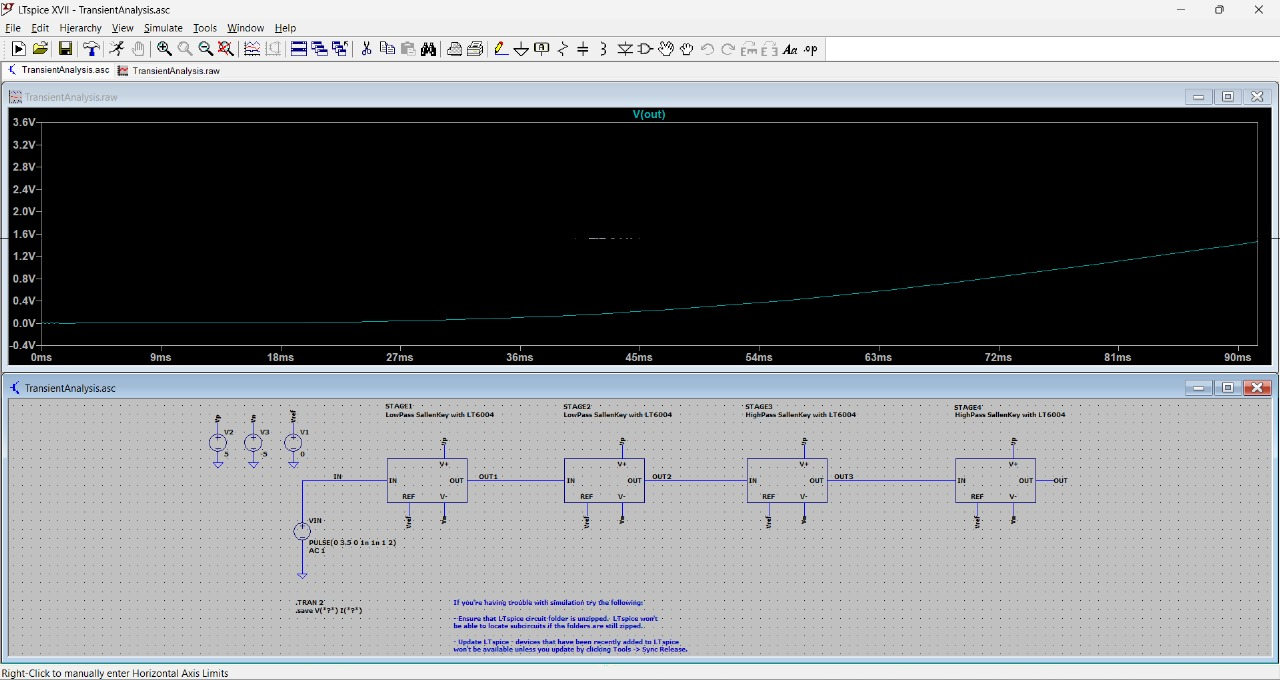
\includegraphics[width=0.95\textwidth]{figures/Trans.jpeg}
  \end{center}
  \caption{Transient analysis of the FIR filter circuit.}
\end{figure}

\begin{figure}[H]
  \begin{center}
    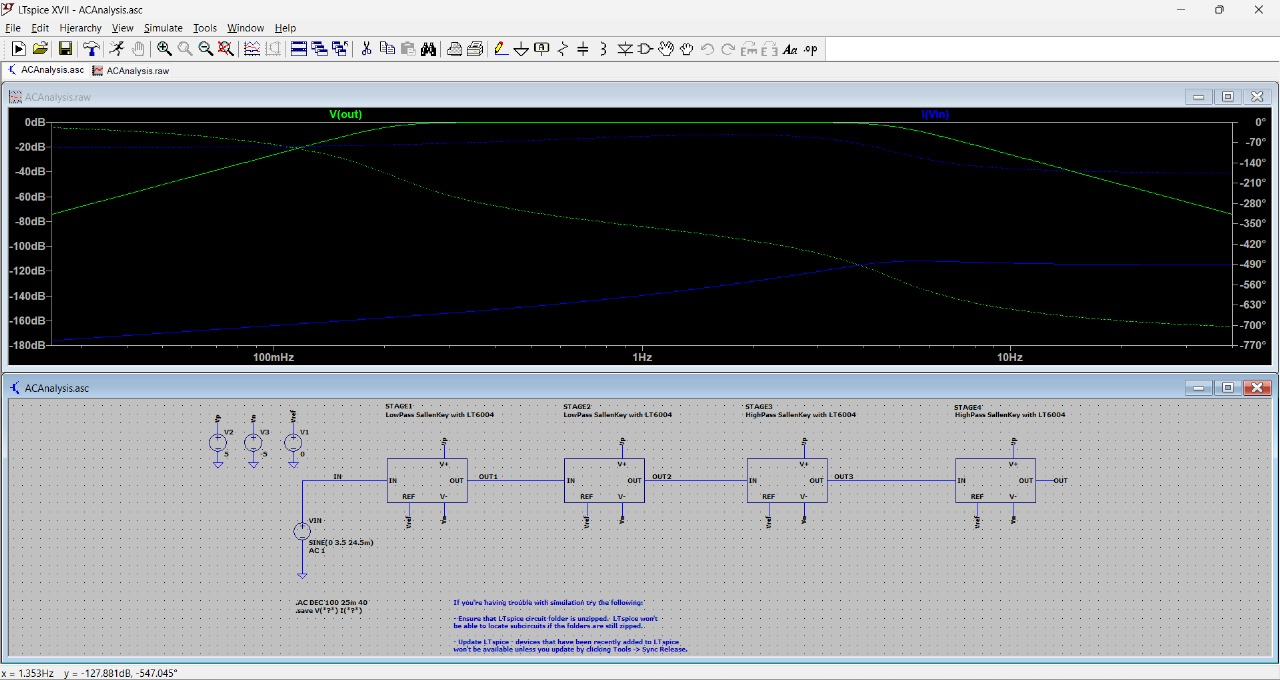
\includegraphics[width=0.95\textwidth]{figures/AC.jpeg}
  \end{center}
  \caption{AC analysis of the FIR filter circuit.}
\end{figure}

\begin{figure}[H]
  \begin{center}
    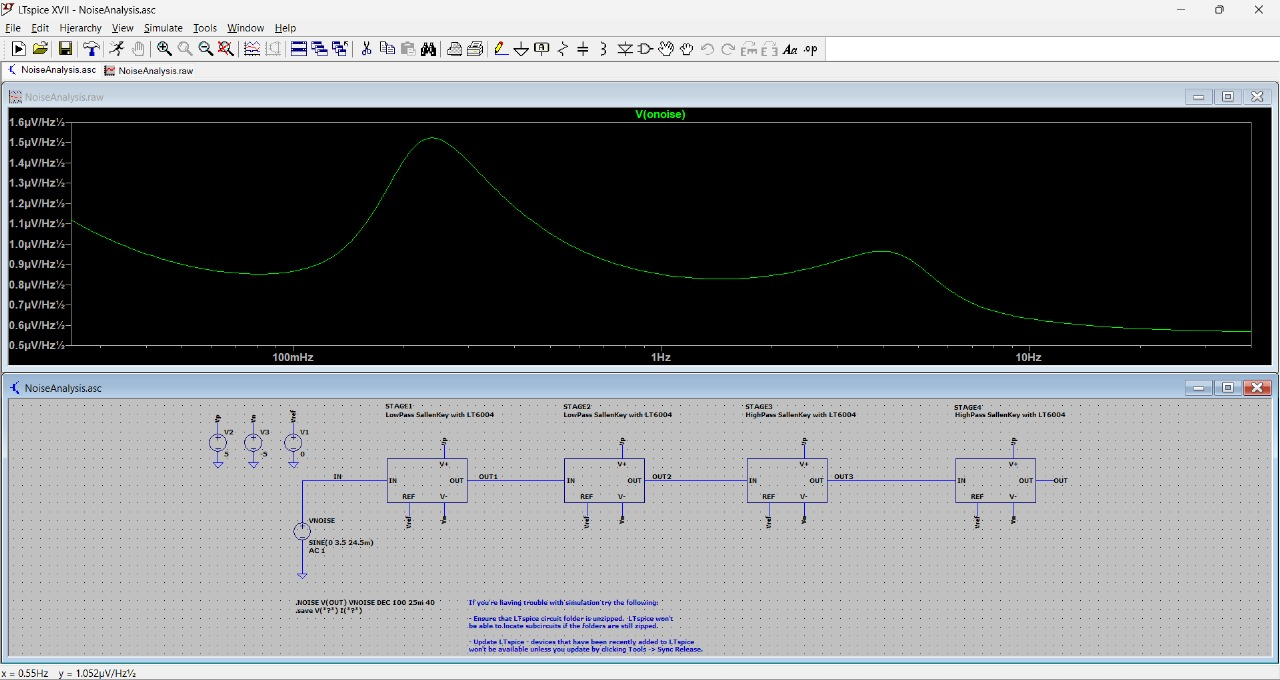
\includegraphics[width=0.95\textwidth]{figures/Noise.jpeg}
  \end{center}
  \caption{Noise analysis of the FIR filter circuit.}
\end{figure}

\subsection{Graphs}
\includepdf[pages=3-12]{figures/Design.pdf}

\end{document}
